\documentclass[main.tex]{subfiles} 

\begin{document}
%%%%%%%%%%%%%%%%%%%%%%%%%%%%%%%%%%%%%%%%%%%%%%%%%%%%%
%%%%%%%%%%%%%%%%    Appendices   %%%%%%%%%%%%%%%%%%%%
%%%%%%%%%%%%%%%%%%%%%%%%%%%%%%%%%%%%%%%%%%%%%%%%%%%%%
\appendix
\section*{Vedlegg 1 - Kartleggingsprøven i sannsynlighetsregning}

Denne kartleggingsprøven (se neste side) ble brukt til å evaluere elever fra 10. trinn
i følgende kompetansemål 
\begin{itemize}
\item finne og diskutere sannsyn gjennom eksperimentering, simulering og berekning i daglegdagse samanhengar og spel
\item beskrive utfallsrom og uttrykkje sannsyn som brøk, prosent og desimaltal
\end{itemize}
\begin{figure}[h!]
  \centering
  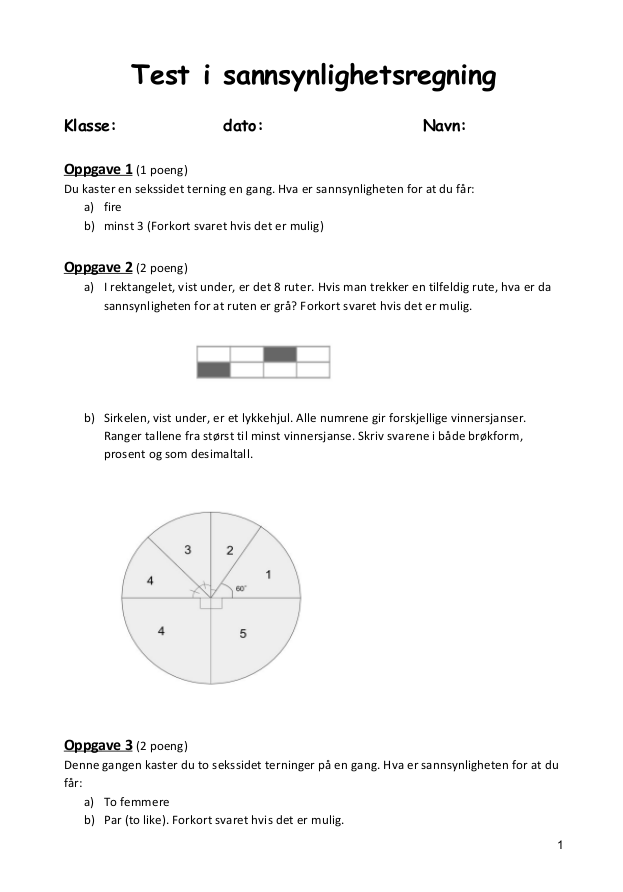
\includegraphics[width=.9\linewidth]{../figures/test1.png}
\end{figure}

\begin{figure}[h!]
  \centering
  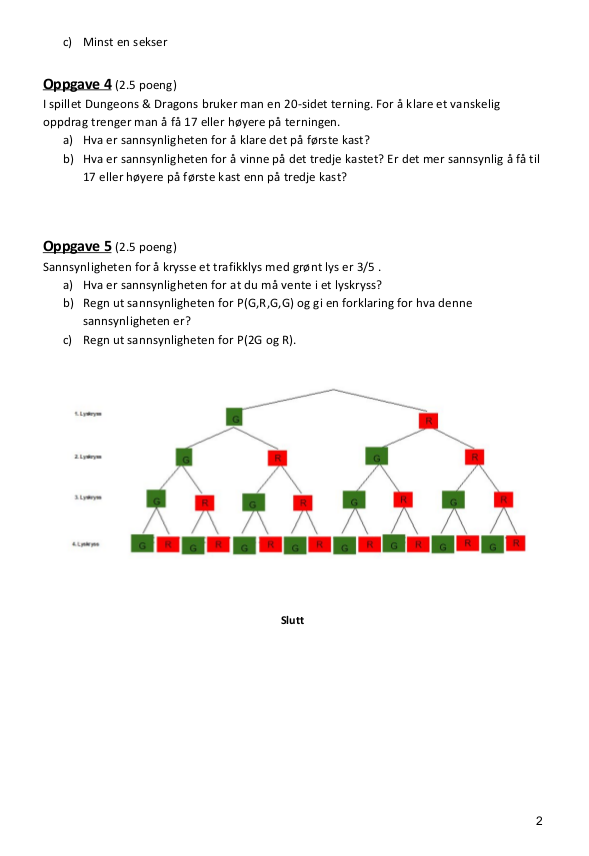
\includegraphics[width=.9\linewidth]{../figures/test2.png}
\end{figure}

\newpage
\section*{Vedlegg 2 - Multiplikasjonsregelen og Addisjonsregelen}

Anta at utfallsrommet til en hendelse, U, er gitt ved 
\begin{align}
U = \{1,2,3,4,5,6\}
\end{align}
Dette kan for eksempel være utfallsrommet til en terningkast. Det vil si alle
mulige utfall som kan forekomme eksisterer i U. Sannsynligheten for at utfallet
terningkast $1$ forekommer er da gitt ved følgende formel
\begin{align}
P(1) &= \frac{\text{antall gunstige utfall}}{\text{antall mulige utfall}} \\
     &= \frac{1}{6}. \nonumber
\end{align}
Da kan vi innføre følgende regler.
\subsection*{Multiplikasjonsregel}
\emph{Sannsynligheten for at flere bestemte uavhengige hendelser inntreffer etter hverandre er lik produktet av 
sannsynlighetene for hver enkel hendelse.}\newline\newline
\textbf{Eksempel}\\
Sannsynligheten for at hendelse $a$ forekommer er $P(a)$ og sannsynligheten for at hendelse $b$ forekommer er
$P(b)$. Da er sannsynligheten for at hendelse $b$ forekommer etter hendelse $b$ gitt ved
\begin{align*}
P(a,b) = P(a)\cdot P(b)
\end{align*}
Det vil si sannsynligheten for hendelse $b$ gitt hendelse $a$ forekommer er gitt ved $P(a,b)$.
\subsection*{Addisjonsregel}
\emph{Sannsynligheten for en kombinert hendelse kan regnes ut ved å legge sammen sannsynligheter for hver enkelt kombinasjon som kan lede til denne hendelsen.}\newline\newline
\textbf{Eksempel}\\
Sannsynligheten for at hendelse $a$ og hendelse $b$ forekommer er gitt ved
\begin{align*}
P(a \text{ og } b) = P(a)\cdot P(b) + P(b)\cdot P(a)
\end{align*}
Det vil si at først forekommer hendelse $a$ og deretter $b$, men hendelse $b$ kan forekomme før hendelse $a$.
Dermed blir sannsynligheten for at både $a$ og $b$ forekommer $P(a \text{ og } b)$.
\end{document}
